% !TeX spellcheck = es_ES
\documentclass[12pt, titlepage]{article}
\usepackage[utf8]{inputenc}
\usepackage[spanish]{babel}
\usepackage{float}
\usepackage[letterpaper, margin=2.5cm]{geometry}
\usepackage[nottoc,notlot,notlof]{tocbibind} % Hace que se agregen las referencias al indice
\usepackage{url}
\usepackage{graphicx} 
\usepackage{listings}
\usepackage{color}
\definecolor{dkgreen}{rgb}{0,0.6,0}
\definecolor{gray}{rgb}{0.5,0.5,0.5}
\definecolor{mauve}{RGB}{253,151,31}

\lstset{frame=tb,
    language=Sql,
    aboveskip=3mm,
    belowskip=3mm,
    showstringspaces=false,
    columns=flexible,
    basicstyle={\small\ttfamily},
    numbers=none,
    numberstyle=\tiny\color{gray},
    keywordstyle=\color{blue},
    commentstyle=\color{dkgreen},
    stringstyle=\color{mauve},
    breaklines=true,
    breakatwhitespace=true,
    tabsize=2,
    morekeywords={use}
}

\title{Reporte: Práctica 1}
\author{Carlos Tonatihu Barrera Pérez \\ Profesor: Hernández Contreras Euler \\ Bases de Datos \\ Grupo: 2CM1 }
\date{3 de marzo de 2017}

\begin{document}
    \maketitle
    \tableofcontents
    \section{Marco Teórico}
    Un \textbf{sistema gestor de bases de datos (SGBD)} consiste en un conjunto de datos interrelacionados y en un conjunto de programas para tener acceso a esos datos. Los datos describen una empresa concreta.
    \\
    El objetivo principal de un \textbf{SGBD} es proporcionar un entorno que sea tanto conveniente como eficiente para las personas que lo usan para la recuperación y almacenamiento de información.
    \\
    Uno de los principales propositos de los sistemas de bases de datos es ofrecer a los usuarios una visión abstracta de los datos. Es decir, el sistema oculta ciertos detalles de la manera en que los datos se almacenan y mantienen.\cite{LIBRO}
    
    Un concepto importante a mencionar son las \textbf{tablas} a las cuales se les asigna un nombre exclusivo De manera burda una tabla es un conjunto de entidades y cada fila es una entidad es por esto que existe una correspondencia entre el termino tabla y el concepto matemático de relación.\cite{LIBRO}
    \\
    Además, es importante mencionar otros conceptos a tratar en esta práctica:
    \begin{itemize}
        \item \textbf{Atributos}. Un atributo hace referencia a las columnas de las tablas.
        \item \textbf{Clave primaria}. Es un campo, o grupo de campos que identifica en forma única un registro. La llave primaria se utiliza para distinguir un registro con el fin de que se pueda  tener acceso a ellos, organizarlos y manipularlos. 
        \item \textbf{Clave foránea}. Es una limitación referencial entre dos tablas la cual identifica una columna o grupo de columnas en una tabla que se refiere a una columna o grupo de columnas en otra tabla.
    \end{itemize}
    \newpage
    \section{Desarrollo}
    En esta practica se comenzó creando la base de datos y seleccionándola para poder usarla. Para realizar esto se usan los siguientes comandos.
    \begin{lstlisting}
    create database trabajos_terminales;
    use trabajos_terminales;
    \end{lstlisting}
    \begin{figure}[H]
        \begin{center}
            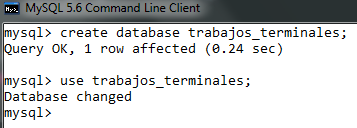
\includegraphics[width=14cm, height=6cm]{img/create.png}
            \caption{Creación y uso de la base.}
            \label{fig:create}
        \end{center}
    \end{figure}
    Se crearon las relaciones con las que se planeaba trabajar, el orden en el que se crean es importante para evitar errores debido a la clave foránea que se usa en dirige y profesor.
    \begin{lstlisting}
    create table tt(
        nott int not null primary key,
        titulo varchar(100)
    );
    
    create table depto(
    idDepto int not null primary key,
    nombre varchar(50)
    );
    
    create table profesor(
        idProf int not null primary key,
        nombre varchar(20),
        ap varchar(30),
        am varchar(30),
        academia varchar(50),
        salario double,
        idDepto int,
        foreign key(idDepto) references depto(idDepto) on delete cascade on update cascade
    );
    
    create table presentacion(
        idPresentacion int not null primary key,
        fecha date,
        califRevisor float,
        califSinodales float,
        tipo varchar(30)
    );
    
    create table dirige(
        idProf int not null,
        nott int not null,
        primary key(idProf, nott),
        foreign key(idProf) references profesor(idProf) on delete cascade on update cascade,
        foreign key(nott) references tt(nott) on delete cascade on update cascade
    );
    \end{lstlisting}
    \begin{figure}[H]
        \begin{center}
            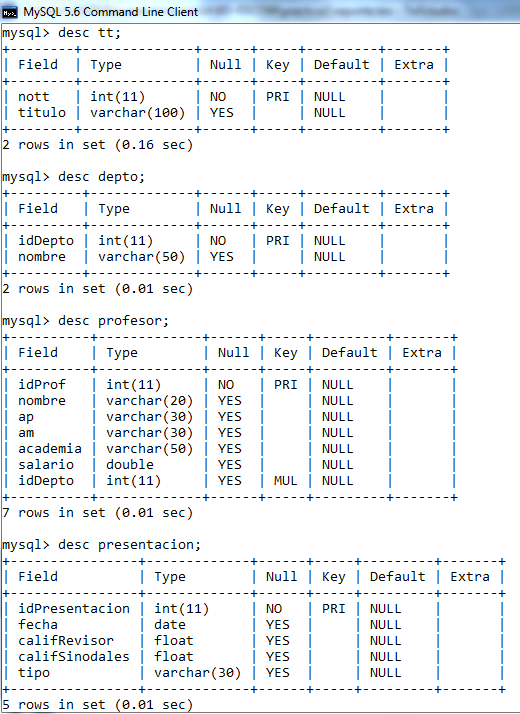
\includegraphics[width=16cm, height=15cm]{img/tablas.png}
            \caption{Descripción de las tablas después de crearlas.}
            \label{fig:tablas}
        \end{center}
    \end{figure}
    En este punto se empezó a modificar la descripción de las tablas usando el comando alter.
    \begin{lstlisting}
    alter table profesor rename as catedratico; -- Esto cambia el nombre de la tabla profesor a catedratico
    alter table presentacion add column dictamen varchar(30); --Agregamos un nueva columna a esta tabla
    alter table depto change column nombre depto varchar(50) not null; -- Se cambia el nombre de la columna 
    alter table catedratico add column tel int; -- Agrega una nueva columna
    alter table catedratico change column tel tel varchar(30); -- Cambia el tipo de dato
    \end{lstlisting}
    \begin{figure}[H]
        \begin{center}
            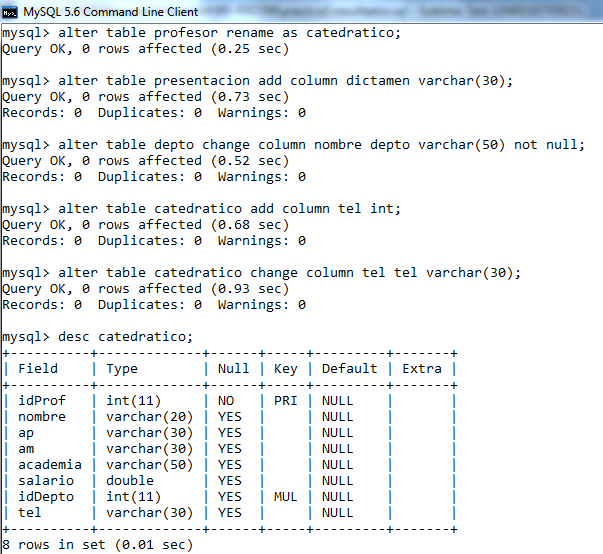
\includegraphics[width=14cm, height=10cm]{img/cambios.png}
            \caption{Cambios en la base.}
            \label{fig:cambios}
        \end{center}
    \end{figure}
\begin{figure}[H]
    \begin{center}
        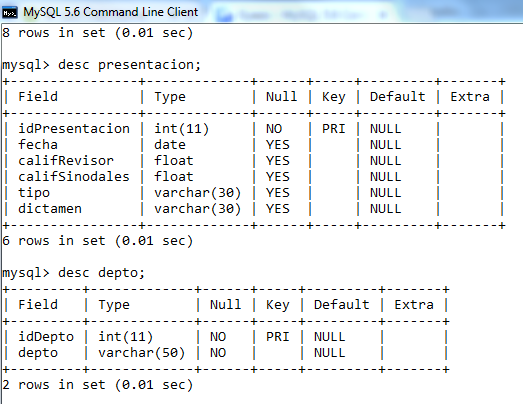
\includegraphics[width=12cm, height=6cm]{img/mascambios.png}
        \caption{Más cambios realizados.}
        \label{fig:cambios2}
    \end{center}
\end{figure}
    Ahora se procedió a agregar una llave foránea a la tabla presentación, para esto primero se creo la columna que seria la futura FK y se especifica con que tabla tiene relación.
    \begin{lstlisting}
    alter table presentacion add column nott int; -- Campo necesario para la foreign key
    alter table presentacion add FOREIGN KEY(nott) references tt(nott)
    on delete cascade on update cascade; -- Creacion de la clave foranea
    \end{lstlisting}
    \begin{figure}[H]
        \begin{center}
            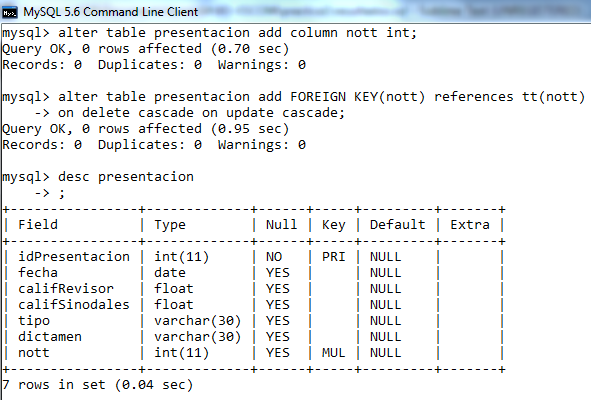
\includegraphics[width=12cm, height=6cm]{img/foranea.png}
            \caption{Creación de la llave foránea}
            \label{fig:foranea}
        \end{center}
    \end{figure}
    Después, se modifico la llave primaria haciéndola compuesta para lograr esto se borra la anterior PK y se agrega la nueva.
    \begin{lstlisting}
    alter table presentacion drop primary key; --Borramos nuestra anterior PK
    alter table presentacion add primary key(idPresentacion, fecha); -- Nueva primary key compuesta
    \end{lstlisting}
    \begin{figure}[H]
        \begin{center}
            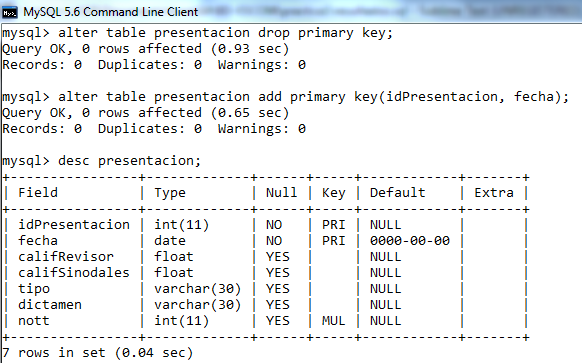
\includegraphics[width=12cm, height=6cm]{img/primaria.png}
            \caption{Creación de la llave primaria compuesta.}
            \label{fig:primaria}
        \end{center}
    \end{figure}
    Finalmente se elimino la clave foránea de una tabla, esto es mas complejo que la llave primaria ya que se debe observar la descripción de la relación para obtener el constraint que tiene asignado dicha clave.
    \begin{lstlisting}
    show create table catedratico; -- Lo usamos para observar el id de la llave foranea
    alter table catedratico drop foreign key catedratico_ibfk_1; -- Ahora si podemos borrar esta llave foranea
    \end{lstlisting}
    \begin{figure}[H]
        \begin{center}
            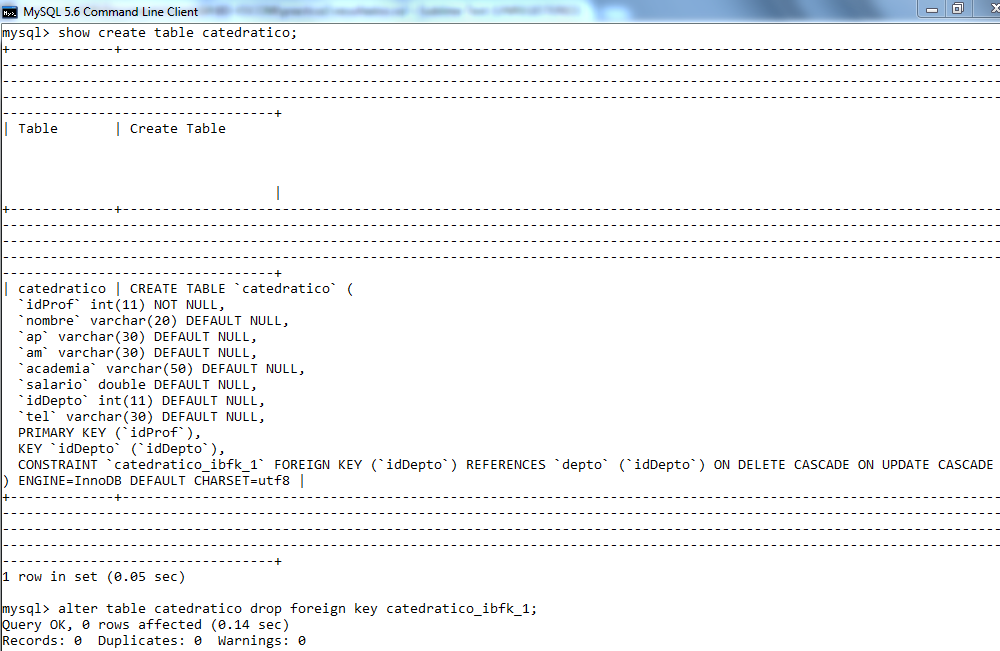
\includegraphics[width=16cm, height=14cm]{img/constraint.png}
            \caption{Se identifico y borro la clave foránea}
            \label{fig:constraint}
        \end{center}
    \end{figure}
\begin{figure}[H]
    \begin{center}
        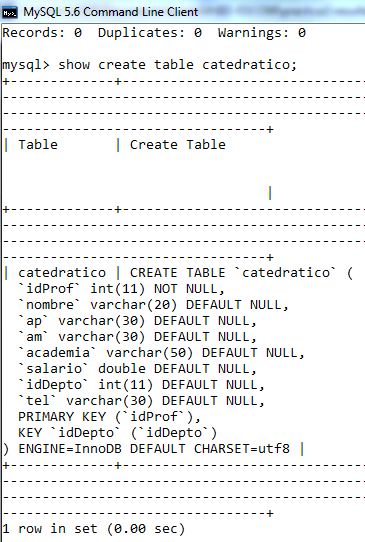
\includegraphics[width=10cm, height=12cm]{img/constraint2.png}
        \caption{Este fue el resultado de borrarlo.}
        \label{fig:constraint2}
    \end{center}
\end{figure}
    Para finalizar se hizo un respaldo, es importante estar en la ruta que se muestra en la imagen para poder realizar esto
    \begin{figure}[H]
        \begin{center}
            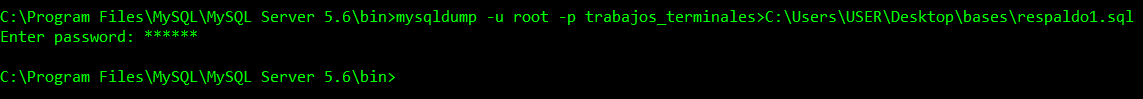
\includegraphics[width=16cm, height=2cm]{img/respaldo.png}
            \caption{Se logro hacer el respaldo sin errores.}
            \label{fig:respaldo}
        \end{center}
    \end{figure}
    \section{Conclusiones}
    Esta primera práctica me permitió empezar a conocer el como se trabaja con una base de datos a un nivel básico pero fundamental también es importante destacar que para dominar esta técnica es necesario seguir practicando y repasando las practicas que se hagan de aquí en adelante.
    \bibliography{bibliografia} 
    \bibliographystyle{ieeetr}
\end{document}